\chapter{Preliminaries}
\label{CH:Preliminaries}

\section{Negligible and non-negligible functions}
\label{SEC:Negligible}
A function $\mu : \nats \to \reals$ is {\it negligible} (in $n$) if it goes to
zero faster than any inverse polynomial $\frac{1}{p(n)}$ in $n$. In other
words, for every $c \in \nats$ there exists an $n_0 \in \nats$ such that
$\mu(n) < \frac{1}{n^c}$ for all $n \geq n_0$. If $\mu$ is not negligible it
is said to be {\it non-negligible} (in $n$). In that case there exists a $d
\in \nats$ such that $\mu(n) > \frac{1}{n^d}$ for infinitely many $n$ (not
necessarily contiguous). 

If definitional robustness is desired, negligible and non-negligible functions
are a natural choice for formalizing the intuitive notions of
``insignificant'' and ``significant'' probabilities when dealing with
polynomial-time adversaries.
%Our interest in non-negligible functions stems from the fact that a
%polynomial-time adversary whose success probability is non-negligible in the
%``security parameter'' $n$ can be transformed via ``parallel repetition'' into a
%polynomial-time adversary whose success probability is exponentially close to
%one (i.e.  bounded below by $1 - \frac{1}{2^n}$). 
%In other words, if a
%polynomial-time adversary whose probability of breaking the security of some primitive of
%interest is merely non-negligible exists, then one whose success probability is
%overwhelming exists also.

\section{One-way functions}
\label{SEC:Oneway}
One-way functions are a cryptographic primitive of fundamental importance. 
%In sections \ref{SEC:Signatures} and \ref{SEC:IDschemes}, respectively, we will see that they
%exist if and only if signature and identification schemes exist.
%They exist if and only if pseudorandom number generators (see
%Section~\ref{SEC:Pseudorandom})
%, which can be used to construct secure
%%private-key encryption schemes (\cite{goldreich:pseudorandom2},
%and secure signature schemes (see Section~\ref{SEC:Signatures}) exist 
%(\cite{hastad:1waytopseudorandom}, \cite{rompel:1waysigs}).
Informally, a function mapping strings to strings is {\it one-way} if it is
``easy to evaluate'' but ``hard to invert on average''. 
Formally, a function $f: \strs{*} \to \strs{*}$ is {\it one-way} if it is
computable in deterministic polynomial time and, for every probabilistic
polynomial-time ``inverter'' $INV$, $p_{INV}(n)$ is negligible. Here
$p_{INV}(n)$ is the probability that, given $1^n$ and $y = f(x)$ for a random $x
\in \strs{n}$, $INV$ outputs an $x' \in \strs{n}$ such that $f(x') = y$;
$p_{INV}(n)$ is taken over the choice of $x \in \strs{n}$ and the random bits
of $INV$.

Observe that if $P = NP$ then every function $f$ computable in deterministic
polynomial time can be easily inverted by non-deterministically guessing an
$x' \in \strs{n}$ 
%in the preimage of $f(x)$. 
such that $f(x') = y$. Proving the existence of one-way functions is therefore no easier
than proving $P \neq NP$.
%
%A permutation is a function $f$ which is both 1-1 (so that $f(x_1) \neq f(x_2)$
%for every $x_1 \neq x_2$) and onto (so that every $y$ in the codomain of $f$ is the
%image of some $x$ in the domain of $f$), also called a bijection or a one-to-one
%correspondence. 
%
%\section{Pseudorandom Number Generators}
%\label{SEC:Pseudorandom}
%Pseudorandom number generators can be used to construct pseudorandom function
%generators, which in turn are the basis of secure private-key cryptosystems
%(\cite{goldreich:pseudorandom1}, \cite{goldreich:pseudorandom2}). Informally,
%a {\it pseudorandom number generator} $G$ is an ``easy to evaluate'' function
%mapping strings of length $n$ to strings of length $\ell(n) > n$ such that the
%distribution over $\ell(n)$-bit strings induced by running $G$ on a random
%$n$-bit string ``looks random'' to polynomial-time adversaries. Another way of
%thinking about this is that the resulting distribution passes all efficient
%``statistical tests for randomness''. The term ``pseudorandom number
%generator'' is in fact a bit of a misnomer, since $G$ as we've defined it is
%actually a pseudorandom {\it string} generator. 
%
%Formally, a function $G: \strs{n} \to \strs{\ell(n)}$ (where $\ell(n)$ can be
%computed in deterministic polynomial time given $1^n$) is a {\it pseudorandom
%number generator} if $G$ is computable in deterministic polynomial time and,
%for every probabilistic polynomial-time ``distinguisher'' $D$ given $1^n$ and
%$\alpha \in \strs{\ell(n)}$, $|p_D(n) - r_D(n)|$ is negligible in $n$.  Here
%$p_D(n)$ is the probability that $D$ accepts $G(s)$ for a random $s \in
%\strs{n}$, whereas $r_D(n)$ is the probability that $D$ accepts a random
%$\alpha$; $p_D(n)$ is taken over the choice of $s \in \strs{n}$ and the random
%bits of $D$, whereas $r_D(n)$ is taken over the choice of $\alpha \in
%\strs{\ell(n)}$ and the random bits of $D$.
%
%It may seem overly restrictive to only allow $D$ to sample the distribution induced
%by $G$ once. Alternatively, we could let $D$ sample it polynomially many
%times; number generators secure against such augmented distinguishers are said to be
%{\it pseudorandom against multiple sampling}. However, a simple ``hybrid argument'' shows that 
%if $G$ is pseudorandom, then it is also pseudorandom against multiple
%sampling (\cite{goldreich:pseudorandom1}). The converse holds trivially.
%
%Notice that every pseudorandom number generator $G$ is a one-way function,
%since otherwise there would exist an efficient distinguisher $D$ which breaks
%the pseudorandomness of $G$. Given $\alpha \in \strs{\ell(n)}$, $D$ simply
%runs the inverter $INV$ on $\alpha$ to obtain a putative seed $s' \in
%\strs{n}$ and accepts if and only if $G(s') = \alpha$. This shows that if
%pseudorandom number generators exist, then so do one-way functions. Recall
%that the converse also holds, as shown in \cite{hastad:1waytopseudorandom}.

\section{Hash function ensembles}
\label{SEC:Hash}
A {\it hash function} $h$ is simply an efficiently-evaluable function mapping
$\strs{*}$ to $\strs{n}$, where $n$ is some security parameter.
``Cryptographic'' hash functions such as SHA-256 (\cite{nist:sha1}) are
informally believed to ``hide all information about their input''. 
More rigorously, hash functions are often assumed to be ``collision resistant'' or
``collision intractable'', meaning that it's infeasible to find two domain
elements which have the same image under $h$.  Formally, however, it doesn't
make sense to assert that collisions in SHA-256 or any other fixed
hash function are hard to find, since they can always be built into the code
of the finder machine. 
%in particular, there exist constant-time machines which output such collisions on any input. 
Instead, we prefer to talk about hash function ensembles.
%a hash function $h$
%is {\it collision resistant} if, for every probabilistic polynomial-time
%``finder'' $F$ who is given $1^n$, the probability $p_F(n)$ that $F$ outputs
%$x_1,x_2 \in \strs{*}$, $x_1 \neq x_2$ such that $h(x_1) = h(x_2)$ is
%negligible; here $p_F(n)$ is taken over the random bits of $F$.

A {\it hash function ensemble} $\fanh = \ens{\fanh}{n}$ is a collection of
hash function families $\fanh_n = \{h_s : \strs{*} \to \strs{n}\}_{s \in
\strs{n}}$\footnote{In general, $h_s$ maps $\strs{*}$ to $\strs{\ell(n)}$,
where $\ell(n) \leq n^c$ for some $c$. However, we will usually assume that $\ell(n) \equiv n$ 
to simplify the presentation.}. $\fanh$ is {\it efficiently
evaluable} in the sense that there exists a (deterministic) polynomial-time
Turing machine $M_\fanh$ such that $M_\fanh(s,x) = h_s(x)$ for all $s \in
\strs{n}$ and $x \in \strs{*}$. We say that $\fanh$ is {\it collision
resistant} if, for every probabilistic polynomial time ``collision finder''
$F$ who is given a randomly chosen $s \in \strs{n}$, the probability $p_F(n)$
that $F$ outputs $x_1,x_2 \in \strs{*}$, $x_1 \neq x_2$ such that $h_s(x_1) =
h_s(x_2)$ is negligible; here $p_F(n)$ is taken over the choice of $s$ and the
random bits of $F$.

It is worth pointing out that collision-resistance implies a kind of
one-wayness (see Section ~\ref{SEC:Oneway}). Suppose that we have a
probabilistic polynomial-time inverter $INV$ who, given a randomly chosen $s
\in \strs{n}$ and $y = h_s(x) \in \strs{n}$ for a randomly chosen $x \in
\strs{n+1}$, outputs with non-negligible (in $n$) probability an $x' \in
\strs{n+1}$ such that $h_s(x') = y$; here the probability is taken over the
choice of $s$ and $x$, as well as the random bits of $INV$. Notice that,
provided $x' \neq x$, $(x,x')$ is a collision in $h_s$. Also, since
$\frac{|\strs{n+1}|}{|\strs{n}|} = 2$, $h_s$ maps two domain elements to each
codomain element on average. We can use $INV$ to
construct a collision finder $F$ as follows. Given a randomly chosen $s \in
\strs{n}$, $F$ randomly chooses (say without replacement) $x_1,\ldots,x_{n^c}
\in \strs{n+1}$ and simulates $INV$ to obtain $x_i' = INV(s,x_i)$, $1 \leq i
\leq n^c$. It can be shown that, if $c$ is ``large enough'', the probability
that there exists an $1 \leq i \leq n^c$ such that $h_s(x_i') = h_s(x_i)$ and
$x_i' \neq x_i$ is non-negligible (in $n$).

\section{Trapdoor permutations}
\label{SEC:Trapdoor}
Impagliazzo and Rudich show in \cite{impagliazzo:nooneway} that proving secure
public-key encryption schemes (see Section~\ref{SEC:PKEPs}) exist assuming
only that one-way functions exist is no easier than proving $P \neq NP$. On
the other hand, if trapdoor permutations exist then so do secure public-key
encryption schemes (\cite{rackoff:cca2}). 

Informally, a bijection mapping $n$-bit strings to $n$-bit strings is a {\it
trapdoor permutation} if it is ``easy to evaluate'' and ``hard to invert on
average'', yet ``easy to invert'' given some additional information.

Formally, a {\it trapdoor permutation} $\fanf$ consists of three polynomial-time
algorithms: a key generator $G$ and two function evaluators, $f$ and $f'$. $G$
is probabilistic, whereas $f$ and $f'$ are both deterministic. Given $1^n$ and
some random bits, $G$ outputs a pair of keys $(k,k')$. Associated with every
pair of keys $(k,k')$ is a pair of functions $(f_k,f'_{k'})$, each mapping
$n$-bit strings to $n$-bit strings; $f_k$ and $f'_{k'}$ are both injective (and
therefore surjective), and $f'_{k'} = f_k^{-1}$. 
%Denote the output of $F$
%given a key $k$ and $s \in \strs{n}$ by $F_k(s)$, and the output of $F'$ given
%a key $k'$ and $s \in \strs{n}$ by $F'_{k'}(s)$. 

For every pair of keys $(k,k')$ generated by running $G$ on $1^n$ (together
with some random bits) and every $x \in \strs{n}$, $f(k,x) = f_k(x)$ and
$f'(k',x) = f'_{k'}(x)$.  Moreover, $f_k$ is a one-way function in the
following sense.  For every probabilistic polynomial-time ``inverter'' $INV$,
$p_{INV}(n)$ is negligible in $n$. Here $p_{INV}(n)$ is the probability that,
given a key $k$ (generated by running $G$ on $1^n$ and some random bits) and
%$F(k,s)$ 
$y = f_k(x) \in \strs{n}$ for a random $x \in \strs{n}$, $INV$ outputs $x =
f'_{k'}(y)$; 
%(there is no need to give $1^n$ to $INV$ since $|F(k,s)| = n$) 
$p_{INV}(n)$ is taken over the choice of $s \in \strs{n}$, as well as the
random bits of $INV$ and $G$ (that is, the choice of $k$).
%\medskip\noindent Specifically, $G$, $F$ and $F^{-1}$ work as follows.
%
%\begin{itemize}
%
%\item Given $1^n$ (together with some random bits), $G$ outputs a pair of
%keys $(k_{f},k_{f^{-1}})$.
%
%\item Given a key $k_f$ and $s \in \strs{n}$, $F$ outputs $F(k_f,s) =
%F_{f}(s) \in \strs{n}$.
%
%\item Given a key $k_{f^{-1}}$ and $s \in \strs{n}$, $F^{-1}$ outputs
%$F^{-1}(k_{f^{-1}},s) = F^{-1}_{f^{-1}}(s) \in \strs{n}$.
%
%\end{itemize}
%
%We insist that for every distinct $s_1,s_2 \in \strs{n}$, 
%$F_f(s_1) \neq F_f(s_2)$ and $F^{-1}_{f^{-1}}(s_1) \neq
%F^{-1}_{f^{-1}}(s_2)$, meaning that the functions 
%defined by $F_f$ and $F^{-1}_{f^{-1}}$ are injective.
%, and
%therefore bijective (since the domain and the codomain are finite sets of
%equal size)
%We also insist that for every $s \in \strs{n}$, $F^{-1}_{f^{-1}}(F_f(s)) =
%s$, meaning that the functions defined by $F_f$ and $F^{-1}_{f^{-1}}$ are
%each other's inverses.
%
%Finally, we require that the function defined by $F_k$ be one-way. Namely, for
%every probabilistic polynomial-time inverter $INV$, the probability
%$p_{INV}(n)$ that given $1^n$, $k_f$ and $F_f(x)$ for a random $x \in
%\strs{n}$ 
%(together with some random bits) 
%$INV$ outputs $x$ is negligible in $n$; $p_{INV}(n)$ is taken over the choice
%of $x \in \strs{n}$, as well as the random bits of $G$ (that is, the choice of
%$k_f$) and $INV$. 

\section{Signature schemes and message authentification codes (MACs)}
\label{SEC:Signatures}
A {\it signature scheme} $SIG$ consists of three polynomial-time algorithms: a
key generator $GEN$, a signer $SIGN$ and a verifier $VER$.  Although in general
all three may be probabilistic, we will assume for convenience that
$GEN$ and $SIGN$ are probabilistic, whereas $VER$ is deterministic (this is
nearly always the case in practice). 

\medskip\noindent
$GEN$, $SIGN$ and $VER$ work as follows.

\begin{itemize}
\item Given $1^n$ and some random bits, 
$GEN$ outputs a pair of keys $(pub,pri)$, where $pub$ is the public key and
$pri$ is the private key. Although in general $|pri| \leq n^c$ for
some $c$,  we will usually assume that $|pri| = n$ to simplify the presentation.

\item Given $1^n$, $pri$, a message $m \in \strs{*}$ and some
random bits, $SIGN$ outputs a signature $\sigma_m \in \strs{p(n)}$ of $m$,
where $p(\cdot)$ is some polynomial. 

\item Given $1^n$, $pub$, a message $m$ and a supposed signature 
$\alpha \in \strs{p(n)}$ or $m$, $VER$ outputs either $1$,
indicating he thinks $\alpha$ is a valid signature of $m$, or $0$, indicating
he thinks it is not.

\end{itemize}
Denote the output of $SIGN$ given $1^n$, $pri$, a message $m$ and some random
bits by $SIGN_{pri}(m)$, and the output of $VER$ given $1^n$, $pub$, $m$ and a
supposed signature $\alpha$ of $m$ by $VER_{pub}(m,\alpha)$.  We require that
$VER$ accept all signatures output by $SIGN$, so that for all $n$, all key
pairs $(pub,pri)$ generated by running $GEN$ on $1^n$ and some random bits,
all messages $m$ and all signatures $\sigma_m = SIGN_{pri}(m)$,
$VER_{pub}(m,\sigma_m) = 1$.

Informally, $SIG$ is {\it secure} if no probabilistic polynomial-time
``forger'' $F$ who knows $pub$ has a significant probability of coming up with
a valid signature $\sigma^*$ of a new message $m^* \in \strs{*}$, even 
%(i.e. one whose signature he hasn't already seen) 
after being shown the signatures of polynomially many messages of his choice.
Since $F$ adaptively chooses the messages whose signatures he is shown and
wins if he successfully signs {\it any} new message (even a ``silly'' one such
as the empty string $\lambda$), this sort of security for signature schemes is sometimes called
``security against existential forgery under adaptive chosen-message attack''. 

Formally, $F$ is equipped with a ``signature oracle'' $\fans$; given a message
$m \in \strs{*}$, $\fans$ outputs a signature $\sigma_m = SIGN_{pri}(m)$ of
$m$.  $SIG$ is {\it secure} if, for every probabilistic polynomial-time forger
$F^\fans$, $p_F(n)$ is negligible in $n$. Here $p_F(n)$ is the probability
that, given $1^n$ and a public key $pub$ (generated by running $GEN$ on $1^n$
and some random bits), $F^\fans$ outputs a pair $(m^*,\sigma^*)$ such that
$\fans$ has not been queried on $m^*$ and $VER_{pub}(m^*,\sigma^*) = 1$;
$p_F(n)$ is taken over the random bits of $GEN$ (that is, the choice of
$(pub,pri)$), $F^\fans_{pub}$ and $VER_{pub}$, as well as the randomness of
$\fans$ (that is, the random bits of $SIGN$).

Building on the results of \cite{goldwasser:signatures2},
\cite{bellare:trapdoorsigs1} and \cite{naor:universal}, Rompel showed in
\cite{rompel:1waysigs} that if one-way functions exist, then so do secure
signature schemes. It's not hard to show that the converse also holds,
namely that if secure signature schemes exist, then so do one-way functions.
Notice that if $SIG$ is a secure signature scheme, then the function $f_{GEN}$
mapping the random bits $r$ of $GEN$ to the public key $pub$ is one-way.
Since $GEN$ runs in polynomial time, $f_{GEN}$ is efficiently evaluable. If
$f_{GEN}$ were easy to invert on average, then a forger $F$ who is given $pub$ could compute
$pri$ with high probability, thereby completely breaking the security of
$SIG$. Thus $f_{GEN}$ is a one-way function. Notice that this means that if
one-way functions do not exist, then neither do secure signatures schemes.
%This shows that if
%secure signature schemes exist, then so do one-way functions.  
%Recall that the
%converse also holds, as shown in \cite{rompel:1waysigs}.

Message authentification codes or MACs, as they are commonly referred to, are
essentially private-key signature schemes. This time there is only one
(private) key, $k$, which is chosen randomly and given to both the signer and
the verifier. As with signature schemes, the standard notion of security for
MACs is ``security against existential forgery under adaptive chosen-message attack''.
Although the forger still has access to a signature oracle $\fans$, this time
he is obviously not given the private key $k$ (which is built into
$\fans$); the forger's success probability is taken over his random bits and
the choice of $k$.

\section{Identification schemes}
\label{SEC:IDschemes}
An {\it identification scheme} $ID$ consists of three probabilistic
polynomial-time algorithms: a key generator $G$, a prover $P$ and a verifier $V$.
$P$ and $V$ are ``linked interactive machines'', meaning that they can
``interact'' by sending messages back and forth between each other.
Informally, $P$'s goal is to convince $V$ that he knows some secret, for
example the private key generated by $G$. Although identification schemes are
interesting in their own right, our interest in them stems from the
fact that they are a source of signature schemes secure in the
ROM (\cite{abdalla:fiatshamirrom}).

Each message exchanged between $P$ and $V$ is called a {\it round}.  If $V$'s
messages consist solely of random bits, then $ID$ is said to be {\it
public-coin}. Three-round, public-coin identification schemes are called {\it
canonical}. This thesis only deals with canonical identification schemes, so
let $ID$ be canonical.  Observe that the prover always goes last, because
otherwise he wouldn't be able to respond to the verifier's last challenge.
Since the prover and the verifier alternate rounds, this means that $P$ first sends a message
to $V$, then $V$ challenges $P$, and finally $P$ responds to $V$'s challenge.

Formally, $ID$ works as follows. First, $G$ is run on $1^n$ and some random
bits to obtain a pair of keys $(PK,SK)$, where $PK$ is the public key and $SK$
is the private key.  Let $P_{SK}$ denote the behaviour of $P$ when given
$1^n$, $SK$ and some random bits, and $V_{PK}$ denote the behaviour of $V$
when given $1^n$ and $PK$.  $P_{SK}$ first sends a {\it commitment}
\textsc{Cmt} to $V_{PK}$, to which $V_{PK}$ replies with a {\it challenge}
\textsc{Ch} consisting of the entire contents of his random tape. $P_{SK}$
then sends a {\it response} \textsc{Rsp} to $V_{PK}$, at which point $V_{PK}$
makes a deterministic decision to either accept or reject (see
Figure~\ref{FIG:CanonicalID}). For reasons which will become clear later, it
is convenient to assume that all of $P_{SK}$'s commitments are of length
$\ell(n)$, where $\ell$ is some polytime-computable function of the security
parameter $n$. This is always the case in practice.

\begin{figure}[htb]
    \centering
    \psfrag{P}{$P$}
    \psfrag{V}{$V$}
    \psfrag{Cmt}{\textsc{Cmt}}
    \psfrag{Ch}{\textsc{Ch}}
    \psfrag{Rsp}{\textsc{Rsp}}
    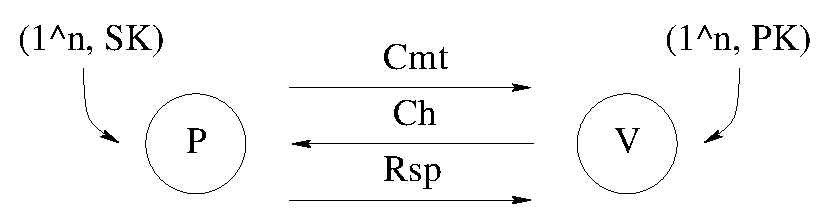
\includegraphics[width = 0.6\textwidth]{../figures/CanonicalIdScheme}
    \caption{The interaction between $P$ and $V$}
    \label{FIG:CanonicalID}
\end{figure}

%When run on input $1^n$, $G$ outputs a pair of keys $(PK,SK)$, where
%$PK$ is the public key and $SK$ is the private key.  
Since the behaviour of $V_{PK}$ is completely determined once his random tape
\textsc{Ch} is fixed, we may think of $V_{PK}$ as a deterministic function
accepting or rejecting ``transcripts'' of the form $(m_1,\textsc{Ch},m_2)$,
where $m_1$ and $m_2$ are the first and second messages received by $V_{PK}$,
respectively; $V_{PK}$ may interact with an adversary who is not $P_{SK}$, so these
need not equal \textsc{Cmt} and \textsc{Rsp}. We require that $P_{SK}$ always
convince $V_{PK}$ to accept, so that
$V_{PK}(\textsc{Cmt},\textsc{Ch},\textsc{Rsp}) = 1$ for all \textsc{Cmt} and
\textsc{Rsp} produced by $P_{SK}$. 

We are interested in two notions of security for identification
schemes: {\it passive security} and {\it active security}.

Informally, $ID$ is {\it passively secure} if no probabilistic polynomial-time
``impersonator'' $I$ who knows $PK$ (but not $SK$)
%given $1^n$ and a public key $PK$ (obtained by
%running $G$ on $1^n$ and some random bits) 
has a 
%non-negligible 
significant probability of convincing $V_{PK}$ to accept when interacting with
him in the role of $P_{SK}$, even after seeing polynomially many transcripts
of conversations between $P_{SK}$ and $V_{PK}$. This weak type of security for
identification schemes is called ``passive'' because $I_{PK}$ passively
monitors the conversation between $P_{SK}$ and $V_{PK}$ without interfering
with it.   

Formally, $I$ is equipped with a ``transcript oracle'' $\fant$. Every time
$\fant$ is queried, it generates a transcript
$(\textsc{Cmt},\textsc{Ch},\textsc{Rsp})$ by running $P_{SK}$ and $V_{PK}$ on
some random bits. $I_{PK}^{\fant}$ is given $1^n$ and a public key $PK$
(generated by running $G$ on $1^n$ and some random bits), together with some
random bits.  $I_{PK}^\fant$ first obtains polynomially many transcripts by
repeatedly querying $\fant$. Next, $I_{PK}^\fant$ sends a commitment
$\textsc{Cmt}'$ to $V_{PK}$, receiving a challenge \textsc{Ch} in reply.
$I_{PK}^\fant$ then responds to the challenge by sending $\textsc{Rsp}'$ to
$V_{PK}$. $ID$ is {\it passively secure} if, for every passive probabilistic
polynomial-time impersonator $I_{PK}^\fant$, the probability $p_I(n)$ that
$V_{PK}(\textsc{Cmt}',\textsc{Ch},\textsc{Rsp}') = 1$ is negligible in $n$;
$p_I(n)$ is taken over the random bits of $G$ (that is, the choice of
$(PK,SK)$), $I_{PK}^\fant$ and $V_{PK}$ (that is, the choice of \textsc{Ch}),
as well as the randomness of $\fant$ (that is, the random bits of $P_{SK}$ and
$V_{PK}$).

Informally, $ID$ is {\it actively secure}, or simply {\it secure}, if no
probabilistic polynomial-time ``impersonator'' $I$ who knows $PK$ (but not
$SK$)
%given $1^n$ and a public key $PK$ (obtained by running $G$ on $1^n$ and some
%random bits) 
has a significant probability of convincing $V_{PK}$ to accept when
interacting with him in the role of $P_{SK}$, even after arbitrarily
interacting with $P_{SK}$ in the role of $V_{PK}$ polynomially many times.
This strong type of security for identification schemes is called ``active''
because $I_{PK}$ actively interacts with $P_{SK}$ rather than merely
monitoring $P_{SK}$'s conversation with $V_{PK}$. 

Formally, we think of $I_{PK}$, who is given $1^n$ and a public key $PK$
(generated by running $G$ on $1^n$ and some random bits), together with some
random bits, as operating in two ``phases''. In the first phase, $I_{PK}$
interacts with $P_{SK}$ (in the role of $V_{PK}$) by sending him polynomially
many adaptively chosen challenges; note that $I_{PK}$ is not constrained to
choose his challenges randomly.
%, but can instead choose them in any way he likes
In the second phase, $I_{PK}$ interacts with $V_{PK}$ (in the role of
$P_{SK}$) as follows. $I_{PK}$ first sends a commitment $\textsc{Cmt}''$ to
$V_{PK}$, receiving a random challenge \textsc{Ch} in reply. $I_{PK}$ then
responds to the challenge by sending $\textsc{Rsp}''$ to $V_{PK}$. $ID$ is
{\it secure} if, for every active probabilistic polynomial-time impersonator
$I_{PK}$, the probability $p_I(n)$ that
$V_{PK}(\textsc{Cmt}'',\textsc{Ch},\textsc{Rsp}'') = 1$ is negligible in $n$;
$p_I(n)$ is taken over the random bits of $G$ (that is, the choice of
$(PK,SK)$), $I_{PK}$, $V_{PK}$ (that is, the choice of \textsc{Ch}) and
$P_{SK}$.

Note that if $V_{PK}$'s challenge $\textsc{Ch}$ is too short,
$|\textsc{Ch}| = \log_2(n)$ say, then the size of the challenge space is only
$2^{|\textsc{Ch}|} = n$. 
%This means that an active impersonator can determine the correct response to
%every possible challenge in polynomial (in fact, linear) time, whereas a
%passive impersonator will receive with non-negligible probability a challenge
%he has already seen the response to. 
An impersonator $I_{PK}$ in possession of even a single valid transcript
$(\textsc{Cmt},\textsc{Ch},\textsc{Rsp})$, obtained through either interacting
with $P_{SK}$ or querying $\fant$, can in this case break the security of $ID$ as
follows. $I_{PK}$ sends \textsc{Cmt} to $V_{PK}$, receives a challenge
$\textsc{Ch}'$ from $V_{PK}$ and sends \textsc{Rsp} to $V_{PK}$ in response. Since $V_{PK}$
accepts whenever $\textsc{Ch}' = \textsc{Ch}$, which happens with probability
$\frac{1}{n}$ (and possibly even if $\textsc{Ch}' \neq \textsc{Ch}$),
$I_{PK}$'s success probability is non-negligible.  In order for $ID$ to hope
to satisfy either of the above two definitions of security, the challenge
space must therefore be of size super-polynomial in $n$, meaning that
$|\textsc{Ch}| = \omega(\log n)$. 

Observe that passive security is strictly weaker than active security, since
every actively secure $ID$ is also passively secure, but not vice versa.
Active security implies passive security because, for every (passive)
impersonator $I_{PK}^\fant$ who breaks the passive security of $ID$, there is
a corresponding (active) impersonator $I_{PK}$ who breaks the active security
of $ID$: $I_{PK}$ simply simulates $I_{PK}^\fant$, taking care to accumulate
enough valid transcripts during the first phase (by choosing the challenges he
sends to $P_{SK}$ randomly) to answer all of $I_{PK}^\fant$'s $\fant$ queries; 
$I_{PK}$'s success probability is identical to that of $I_{PK}^\fant$. 

To see that passive security does {\it not} imply active security, consider
the following (admittedly rather contrived) modification $ID'$ of an arbitrary passively secure
identification scheme $ID$ (such identification schemes exist if one-way
functions do, as we'll see below); we may assume without loss of generality that
$|\textsc{Ch}| = n$. $ID'$ is identical to $ID$, except that whenever the new
prover $P_{SK}'$ receives the challenge $\bar{0} = 0^n$, he responds by
revealing the private key $SK$. $ID'$ remains passively secure, since a
passive impersonator $I_{PK}^\fant$ whose running time is bounded above by
some polynomial $p(\cdot)$ in the security parameter $n$ will see a transcript
containing $SK$ with probability at most $\frac{p(n)}{2^n}$, which is
negligible. However, it is completely trivial for an active impersonator
$I_{PK}$ to break the (active) security of $ID'$: $I_{PK}$ sends $\bar{0}$ to
$P_{SK}'$ to obtain the secret key $SK$ in the first phase, then simulates
$P_{SK}'$ in order to correctly respond to $V_{PK}'$'s challenge in the second phase.

Finally, observe that secure identification schemes exist if and only if
one-way functions do. To see that if secure identification schemes exist then
so do one-way functions, let $ID = (G,P,V)$ be an arbitrary secure canonical
identification scheme. The function $f_{G}$ mapping the random
bits $r$ of $G$ to the public key $PK$ must be one-way, since otherwise an
impersonator could completely break the security of $ID$ (see
Section~\ref{SEC:Signatures}). To see that secure canonical identification
schemes exist if one-way functions do, we need only show how to convert
an arbitrary secure signature scheme into a secure canonical identification
scheme (recall that secure signature schemes exist if one-way functions do). 

We can easily obtain a canonical identification scheme $ID = (G,P,V)$ from any
signature scheme $SIG = (GEN,SIGN,VER)$; $V$ simply challenges $P$ to sign a
random $n$-bit message \textsc{Ch} and accepts only if \textsc{Rsp} is a valid
signature of \textsc{Ch}. Specifically, $G$ is the same as
$GEN$ (so that $(pub,pri) = (PK,SK)$), \textsc{Cmt} = $\lambda$, \textsc{Rsp}
= $SIGN_{SK}(\textsc{Ch})$ and $V_{PK}(\lambda,\textsc{Ch},\textsc{Rsp}) =
VER_{PK}(\textsc{Ch},\textsc{Rsp})$. 

It's not too hard to see that if $SIG$ is secure (as a signature scheme) then
$ID$ is secure (as an identification scheme). An active
impersonator $I$ which successfully breaks the security of $ID$ first gets to
see the signatures of polynomially many messages of his choice and then
successfully signs a random message \textsc{Ch}, whose signature he almost
certainly hasn't already seen (because the challenge space is of
super-polynomial size); a polynomial-time forger $F^\fans$ with access to a
signature oracle $\fans$ can easily simulate $I$, thereby breaking the security
of $SIG$. 
%This means that if one-way functions exist then so do secure
%canonical identification schemes, because secure signature schemes exist if
%one-way functions do.

\section{Public-key encryption schemes}
\label{SEC:PKEPs}
A {\it public-key encryption scheme} $PKE$ consists of three 
polynomial-time algorithms: a key generator $GEN$, an encryptor $ENC$ and a
decryptor $DEC$. $GEN$ and $ENC$ are probabilistic (our definition of security
will crucially depend on the fact that $ENC$ is probabilistic), whereas
$DEC$ is deterministic. 

Informally, the setup is that a person $A$ wants to securely communicate with
some stranger $B$ he knows nothing about, except for his name and address.  To
this end, $A$ generates a pair of keys $(pub,pri)$ using $GEN$, sends the public
key $pub$ to $B$ and keeps the private key $pri$ for himself.  To communicate
a message $m$ to $A$, $B$ obtains an encryption $e_m$ of $m$ using $ENC$ and
sends $e_m$ to $A$; $A$ then decrypts $e_m$ using $DEC$. 
%Security in this
%setting means that no probabilistic polynomial-time adversary $ADV$ who is
%given $pub$ and $e_m$ (but not $pri$) can ``learn'' any information about $m$,
%even after seeing the decryptions of polynomially many messages of his choice.
%
%Observe that communication between $A$ and $B$ as we've defined it is
%unidirectional ($B$ only talks and $A$ only listens), whereas we would like
%$A$ and $B$ to have a normal conversation. One way to accomplish this is for
%$B$ to generate his own pair of keys $(pub',pri')$ using $GEN$ and send $pub'$
%to $A$.  However, that isn't necessary in practice, since $B$ can simply send
%an encryption of a random key $k$ to $A$. Once $A$ and $B$ share a random key,
%they can securely communicate using ``private-key encryption''. In other
%words, public-key encryption schemes can be used for ``secure key exchange''.
%, though the standard notions of security are in some sense ``overkill'' in that case.

For reasons of modularity and efficiency, public-key encryption schemes are in
practice almost always used solely to securely exchange a ``short'' private
key $k$, whose length we'll assume to be equal to the security parameter $n$
for convenience. Once both $A$ and $B$ are in possession of $k$, they can
securely communicate using highly efficient ``private-key encryption''. Thus,
unlike in the case of signature schemes, where we insisted that
$SIGN$ be able to sign messages of arbitrary length, here we will only require
$ENC$ to be able to encrypt $n$-bit messages.  

Formally, $GEN$, $ENC$ and $DEC$ work as follows.

\begin{itemize}

\item Given $1^n$ and some random bits, $GEN$ outputs a pair of keys
$(pub,pri)$, where $pub$ is the public key and $pri$ is the private key.

\item Given $1^n$, $pub$, a message $m \in \strs{n}$ and some random bits,
$ENC$ outputs an encryption $e_m \in \strs{p(n)}$ of $m$, where $p(\cdot)$ is
some polynomial.

\item Given $1^n$, $pri$ and a supposed encryption $\alpha$, $DEC$ either
outputs a message $m \in \strs{n}$ or a special symbol $\bot$ indicating a
failure to decrypt.

\end{itemize}
Denote the output of $ENC$ given $1^n$, $pub$, $m \in \strs{n}$ and some random
bits by $ENC_{pub}(m)$, and the output of $DEC$ given $1^n$, $pri$ and 
$\alpha \in \strs{p(n)}$ by $DEC_{pri}(\alpha)$.  We require that $DEC$
correctly decrypt all encryptions produced by $ENC$, so that for all $n$, all
key pairs $(pub,pri)$ generated by running $GEN$ on $1^n$ and some random bits,
all messages $m \in \strs{n}$ and all encryptions $e_m = ENC_{pub}(m)$,
$DEC_{pri}(e_m) = m$. 

We are interested in two notions of security for public-key encryption
schemes: {\it semantic security} and {\it chosen-ciphertext security}.

Informally, $PKE$ is {\it semantically secure} (\cite{goldwasser:probenc2}) if
no probabilistic polynomial-time ``eavesdropper'' $E$ who knows $pub$ (but not
$pri$) and passively monitors the channel between $A$ and $B$ can ``learn''
even a single bit of information about a message $m$ through seeing its
encryption $e_m$. 

Formally, $E$ is given $1^n$ and a public key $pub$ (generated by running
$GEN$ on $1^n$ and some random bits) and chooses two distinct $n$-bit
messages, $m_0$ and $m_1$. A bit $b$ is then chosen randomly (but not shown to
$E$), and $E$ is given an encryption $e_b = ENC_{pub}(m_b)$ of $m_b$. $E$ next
computes for a while, finally outputting a bit $b'$. Let $p_{E}(n)$ be the
probability that $b' = b$, meaning that $E$ correctly determined $b$;
$p_{E}(n)$ is taken over the random bits of $E$ and $GEN$ (that is, the choice
of $(pub,pri)$), as well as the choice of $b$.  $PKE$ is {\it semantically
secure} if, for every probabilistic polynomial-time eavesdropper $E$,
$|\frac{1}{2} - p_{E}(n)|$ is negligible in $n$ (in other words, $p_{E}(n)$
doesn't significantly differ from $\frac{1}{2}$, the probability of randomly
guessing $b$).

Note that $PKE$ cannot be semantically secure if $ENC$ is deterministic. In
order to break the semantic security of $PKE$, an eavesdropper
$E$ (who knows $pub$) simply computes $\eta_0 = ENC_{pub}(\bar{0})$ and
$\eta_1 = ENC_{pub}(\bar{1})$, where $\bar{0} = 0^n$ and $\bar{1} = 0^{n-1}1$,
then sets $m_0 = \bar{0}$ and $m_1 = \bar{1}$.  Once $E$ receives $e_b$, he
outputs 0 if $e_b = \eta_0$ and 1 if $e_b = \eta_1$ (these are the only two
possibilities because $ENC$ is deterministic). Since $E$ always outputs $b$
correctly (so that $b' = b$ with probability 1), $|\frac{1}{2} - p_E(n)| =
\frac{1}{2}$, which is certainly non-negligible.
 
Informally, $PKE$ is {\it secure against (adaptive) chosen-ciphertext attack}
or {\it CCA2-secure} (\cite{rackoff:cca2}) if no probabilistic polynomial-time
adversary $ADV$ who knows $pub$ (but not $pri$) and has complete control over
the channel between $A$ and $B$ can ``learn'' even a single bit of information
about a message $m$ through seeing its encryption $e_m$. What does it mean for
$ADV$ to have ``complete control'' over the channel between $A$ and $B$?
Intuitively, $ADV$ intercepts all encryptions or ``ciphertexts'' sent by $A$
to $B$ and sends $B$ whatever he likes instead.

Formally, $ADV$ is given $1^n$ and a public key $pub$ (generated by running
$GEN$ on $1^n$ and some random bits) and equipped with a ``decryption oracle''
$\fand$, which outputs $DEC_{pri}(\alpha)$ when queried on a ciphertext
$\alpha \in \strs{p(n)}$.  $\fand$ is meant to capture the intuition that
$ADV$ can effectively force $B$ to decrypt any ciphertext of his choosing (of
course the answer may well be $\bot$; we think of ``ciphertexts'' that decrypt
to $\bot$ as being malformed).

$ADV^\fand$ queries $\fand$ on $\alpha_0$ and receives $DEC_{pri}(\alpha_0)$,
queries $\fand$ on $\alpha_1$ and receives $DEC_{pri}(\alpha_1)$, and so on.
Since $ADV^\fand$ may in general choose his queries based on $\fand$'s
previous answers, this is an adaptive attack.  Eventually, $ADV^\fand$ chooses
two distinct $n$-bit messages, $m_0$ and $m_1$. A bit $b$ is then chosen
randomly (but not shown to $ADV^\fand$), and $ADV^\fand$ is given an
encryption $e_b = ENC_{pub}(m_b)$ of $m_b$. 

$ADV^\fand$ now gets to query $\fand$ on some additional ciphertexts, whose
choice may in general depend on $e_b$.  Naturally, we don't allow $ADV^\fand$
to query $\fand$ on $e_b$ itself, since $DEC_{pri}(e_b)$ uniquely determines
$b$ (because $m_0 \neq m_1$). Alternatively, once $ADV^\fand$ receives $e_b$
we could forbid him from querying $\fand$ altogether; security against this
type of ``lunchtime attack'' is called {\it CCA1 security} (\cite{naor:cca1}).
However, that would arguably be too restrictive, since in practice CCA2
security is almost always broken by querying $\fand$ on ciphertexts ``related
to'' (though not the same as) $e_b$.

$ADV^\fand$ next computes for a while, finally outputting a bit $b'$.  Let
$p_{ADV}(n)$ be the probability that $b' = b$, meaning that $ADV^\fand$
correctly determined $b$; $p_{ADV}(n)$ is taken over the random bits of
$ADV^\fand$ and $GEN$ (that is, the choice of $(pub,pri)$), as well as the
choice of $b$ (the decryption oracle $\fand$ is deterministic).
$PKE$ is {\it CCA2 secure} if, for every probabilistic polynomial-time
adversary $ADV^\fand$, $|\frac{1}{2} - p_{ADV}(n)|$ is negligible in $n$ (in
other words, $p_{ADV}(n)$ doesn't significantly differ from $\frac{1}{2}$, the
probability of randomly guessing $b$).

Observe that semantic security is strictly weaker than CCA2 security, since
every CCA2-secure $PKE$ is also semantically secure, but not vice versa. CCA2
security implies semantic security because, for every eavesdropper $E$ who
breaks the semantic security of $PKE$, there is a corresponding adversary
$ADV^\fand$ who breaks the CCA2 security of $PKE$: $ADV^\fand$ simply
simulates $E$, ignoring the decryption oracle $\fand$; $ADV^\fand$'s success
probability is identical to that of $E$. This implies that $PKE$ cannot be
CCA2-secure if $ENC$ is deterministic --- we already know that such a $PKE$ is
not semantically secure, and we just showed every CCA2-secure public-key
encryption scheme is.

To see that semantic security does {\it not} imply CCA2 security, consider the
following (admittedly rather contrived) modification $PKE'$ of an arbitrary
semantically secure public-key encryption scheme $PKE$. $PKE'$ is identical to
$PKE$, except that the new encryptor $ENC'$ appends an additional bit, say 0
for concreteness, to every encryption; this bit is ignored by the new
decryptor $DEC'$. $PKE'$ remains semantically secure, since, for every
eavesdropper $E'$ who breaks the semantic security of $PKE'$, there is a
corresponding eavesdropper $E$ who breaks the semantic security of $PKE$: $E$
simulates $E'$ to obtain a pair of messages $(m_0,m_1)$, receives
an encryption $e_b$ and gives $e_b 0$ to $E'$, accepting if and only if $E'$
accepts; $E$'s success probability is identical to that of $E'$. 

However, it is completely trivial for an adversary $ADV^\fand$ to break the
CCA2 security of $PKE'$: $ADV^\fand$ sets $m_0 = \bar{0}$ and $m_1 = \bar{1}$,
receives $e_b = ENC'_{pub}(m_b)$, and queries $\fand$ on $e_b 1$ to obtain a
decryption $m'$. He then outputs $0$ if $m' = \bar{0}$ and $1$ if $m' =
\bar{1}$ (these are the only two possibilities, since $DEC'$ ignores the
trailing bit). Since $ADV^\fand$ always outputs $b$ correctly (so that $b' =
b$ with probability 1), $|1 - p_{ADV}(n)| = \frac{1}{2}$, which is certainly
non-negligible.  Although our highly artificial modification of $PKE$ may seem
like a cheat, in practice public-key encryption schemes fail to be CCA2-secure
for the same reason as $PKE'$. Namely, they are ``malleable'', which
informally means that an adversary $ADV^\fand$ can ``malleate'' (that is,
modify) $e_b$ into some related encryption $e'_b$ such that $b$ can be
computed from $\fand(e'_b)$ ($ADV^\fand$ is allowed to query $\fand$ on $e_b'$
since $e_b' \neq e_b$).

\section{The Random Oracle Model (ROM)}
\label{SEC:ROM}
The Random Oracle Model, or ROM for short, is a setting where all parties have
access to a ``random oracle'' $\fanr$. The ROM was formally introduced
in the context of cryptography in \cite{bellare:rompractical}. 

One way to think of $\fanr$ is as a randomly chosen function mapping
$\strs{*}$ to $\strs{n}$\symbolfootnote[2]{In general, $\fanr$ maps $\strs{*}$
to $\strs{\ell(n)}$, where $\ell(n) \leq n^c$ for some $c$. However, we will
usually assume that $\ell(n) \equiv n$ to simplify the presentation.}.
%, where $p(\cdot)$ is some polynomial in the security
%parameter $n$ (for convenience, we often assume that
%assume without loss of generality
%$p(n) \equiv n$). 
However, the set of all such functions is (countably)
infinite, and we prefer not to talk about sampling such sets.
%it doesn't formally make sense to talk about sampling infinite sets in this
%case. 
Instead, we view $\fanr$ as choosing his answers ``on-line''.  When
queried on $q \in \strs{*}$, $\fanr$ first checks whether $q$ is a ``new
query'', meaning that he hasn't been queried on $q$ before. If so, he randomly
chooses a response $ans \in \strs{n}$ to $q$, writes $ans$ down somewhere
and then outputs it.  Otherwise (namely in the case that $\fanr$ has been
queried on $q$ already), he looks up and outputs his previous response to $q$;
this ensures that identical queries receive an identical response (which is
the case when $\fanr$ is viewed as a function).  
%Although in this way $\fanr$'s responses are not ``filled-in'' until the
%corresponding queries are asked, the resulting distribution over responses
%agrees with our intuition about randomly choosing $\fanr$ from among all
%functions mapping $\strs{*}$ to $\strs{p(n)}$.

We next show that, in some appropriate sense at least, random oracles are
one-way (see Section~\ref{SEC:Oneway} for a definition of one-wayness).  Let
$p_{INV}(n)$ denote the probability that a probabilistic polynomial-time
inverter $INV^\fanr$ who 
%has oracle access to $\fanr$ and 
is given $y = \fanr(x) \in \strs{n}$ for a randomly chosen $x \in \strs{n}$
outputs an $x' \in \strs{n}$ such that $\fanr(x') = y$; $p_{INV}(n)$ is taken
over the choice of $x$, the random bits of $INV^\fanr$ and the randomness of
$\fanr$. Observe that $y$ yields no information about $x$, since it is
distributed uniformly over $\strs{n}$ no matter what $x$ is. Denote the
strings $INV^\fanr$ queries $\fanr$ on by $x_1,\ldots,x_{q_\fanr}$, and set
$y_i = \fanr(x_i)$ for $1 \leq i \leq q_\fanr$;
%$INV^\fanr$'s best strategy is therefore to choose as many distinct strings
%$x_i \in \strs{n}$ as possible, query $\fanr$ on each $x_i$ to obtain $y_i =
%\fanr(x_i)$, and hope that there exists an $i$ such that $y_i = y$.  Denote
%the number of times $INV^\fanr$ queries $\fanr$ by $q_\fanr$, 
notice that $q_\fanr \leq n^c$ for some $c$,
because $INV^\fanr$ runs in (strict) polynomial time. $INV^\fanr$ wins if
there is an $1 \leq i \leq q_\fanr$ such that either $x_i = x$ or $x_i \neq x$
but $y_i = y$ anyway. Applying the union bound, we see that this happens with probability at most
$\frac{2q_\fanr}{2^n} \leq \frac{2n^c}{2^n}$, which is negligible.
%For every $1 \leq j \leq
%q_\fanr$, we have:
%\begin{align*}
%\text{Pr}[y_j = y] &= \text{Pr}[y_j = y \mid x_j = x]\cdot\text{Pr}[x_j = x] 
%+ \text{Pr}[y_j = y \mid x_j \neq x]\cdot\text{Pr}[x_j \neq x] \\ &=
%\frac{1}{2^n - (j-1)} + \frac{1}{2^n}\left(1 - \frac{1}{2^n - (j-1)}\right)
%\leq \frac{1}{2^n - (j-1)} + \frac{1}{2^n} \\ &\leq \frac{2}{2^n - j + 1}
%\leq \frac{2}{2^n - q_\fanr + 1} \end{align*} Applying the union bound then
%gives $p_{INV}(n) \leq \frac{2q_\fanr}{2^n - q_\fanr + 1} \leq
%\frac{2n^c}{2^n - n^c + 1}$, which is negligible in $n$.  \[ \text{Pr}[x = x'
%\mid y = y'] = \frac{1}{2^{p(n)}} \text{ for all } x' \in \strs{n} \text{ and
%}y' \in \strs{p(n)},
%\]
%so that $y$ yields no information about $x$ (here the probability is taken
%over the choice of $x$ and the randomness of $\fanr$). 
%This means that $p_{INV}(n) \leq
%\frac{q_\fanr}{2^{p(n)}} \leq \frac{n^c}{2^{p(n)}}$, which is negligible in
%$n$.

